We used a number of tests to validate the code. 
\section{Matrix Properties}
Since we are using a finite element approximation, the left hand side should be symmetric positive definite. I implemented a unit test to check for this property.

\section{Hand Calculated Problems}
Hand calculated solutions, although tedious to compute, proved to be the most helpful in debugging. I computed solutions to a two element problem (one with a square domain and one rectangular) as well as an eight element problem. These calculations were done in a jupyter notebook that is included with the code. 

\section{No Scattering}
We tested the no scattering case with one material and one energy group. The absorption cross section and the external source were both set to 10. The expected answer was a scalar flux of one in the center. 

\section{Scattering}
To test the code's ability to handle scattering, we chose a simple test problem.  In an infinite medium we can assume no gradient, so the diffusion equation will equal $\phi \approx \frac{q}{\sigma_a}$ in the center. In our test, the absorption cross section was set to two and the external source was ten, meaning $\frac{q}{\sigma_a} = 5$. In the test problem, we have a much smaller domain, so there will be leakage, but the flux in the center should still be close to $\frac{q}{\sigma_a}$ We expect a flux of $\approx 5$ in the center. 

\section{Multigroup Scattering, No Upscatter}
To test the Gauss-Seidel multigroup scattering method we use the two group diffusion equation as a benchmark. 
\begin{align}
 D_1\nabla^2 \phi_1 - \Sigma_{r, 1 \rightarrow 1} \phi_1 + s_1^{'''} &= 0 \\
 D_2\nabla^2 \phi_2 - \Sigma_{r, 2 \rightarrow 2} \phi_2 + s_2^{'''} + \Sigma_{s, 1 \rightarrow 2} \phi_1 &= 0
\end{align}

where $D_g = \frac{1}{3\Sigma_{t, g}}$ and $\Sigma_{r, g \rightarrow g} = \Sigma_{t, g} - \Sigma_{s, g \rightarrow g}$. In an infinite medium we can assume no gradient, so the flux should approach $\frac{s_1^{'''}}{\Sigma_{r, 1}}$ in the first energy group and $\frac{s_2^{'''} + \phi_1 \Sigma_{s, 1 \rightarrow 2}}{\Sigma_{r, 2}}$ in the second.  

This problem was run with $ s^{'''} = 1$ for both groups, $\Sigma_{s, 1\rightarrow 2} = 11$, $\Sigma_{r, 1} = 2$ and $\Sigma_{r, 2} = 1$ This gives an expected flux of $0.50 $ in the first group and $1.50$ in the second. 

\section{NDA/SAAF Agreement}
As the SAAF equation is non-conservative, it's solution does not necessarily agree with the low order equation it is coupled with. However, the two solutions should approach each other as the number of mesh cells increases \cite{Wang2013}. Our code replicates this behavior. 
\begin{figure}
    \centering
    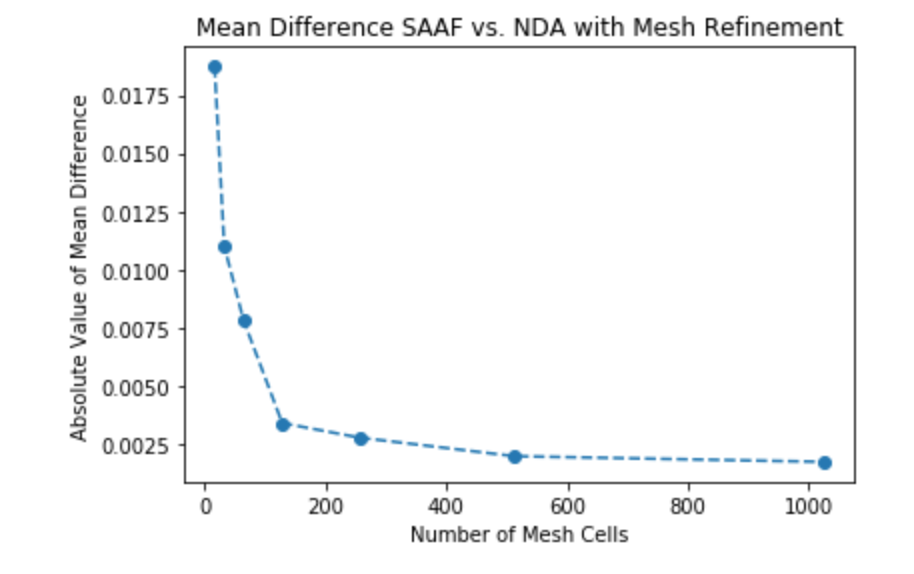
\includegraphics[width=.75\textwidth]{fig/SAAFvsNDA}
    \caption{SAAF/NDA Agreement with Mesh Refinement}
    \label{fig:SAAFvsNDA}
\end{figure}